%!TEX TS-program = xelatex
\documentclass[]{friggeri-cv}

\usepackage{afterpage}
\usepackage{hyperref}
\usepackage{color}
\usepackage{xcolor}
\definecolor{myblue}{RGB}{4, 98, 249}
\usepackage{hyperref}
\hypersetup{
    pdftitle={},
    pdfauthor={},
    pdfsubject={},
    pdfkeywords={},
    colorlinks=true,       % no lik border color
    allbordercolors=white    % white border color for all
}
\addbibresource{bibliography.bib}
\RequirePackage{xcolor}
\definecolor{pblue}{HTML}{0395DE}


% ------------
\usepackage{enumitem}
\renewenvironment{entrylist}{%
  \begin{itemize}[leftmargin=1in]%[leftmargin=*,align=left,itemindent=-\dimexpr\labelwidth+\labelindent+\labelsep\relax]
  }{%
  \end{itemize}
}
\renewcommand{\bfseries}{\headingfont\color{headercolor}}
\renewcommand{\entry}[4]{%
\item[#1]
  \textbf{#2}%
  \hfill%
  {\footnotesize\addfontfeature{Color=myblue} #3}\\%
  #4\vspace{\parsep}%
}
% -------


\begin{document}
\header{Boyang}{Yan}

     
% Fake text to add separator      
\fcolorbox{white}{gray}{\parbox{\dimexpr\textwidth-2\fboxsep-2\fboxrule}{%
.....
}}

% In the aside, each new line forces a line break
\begin{aside}
  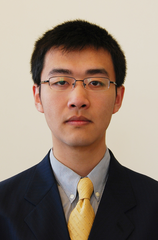
\includegraphics[scale=0.07]{img/boyang.png}
  \section{Address}
  14-6-602 Zhuhuali Community, Huayuanxincheng
  Nankai District,  Tianjin,
  China
    ~
  \section{Contact Info}
  \textbf{Tel:} +86 18512290791
    \textbf{Skype:} yanboyang
    \textbf{Wechat:} yanboyang713
    ~
  \section{Mail}
    \href{mailto:by932@uowmail.edu.au}{\textbf{by932@}\\uowmail.edu.au}
    \href{mailto:yanboyang713@gmail.com}{\textbf{yanboyang713@}\\gmail.com}
    ~
  \section{Web \& Git}
    \href{https://github.com/yanboyang713}{github.com/yanboyang713}
    \href{http://www.yanboyang.com}{yanboyang.com}
    ~
  \section{Programming}
    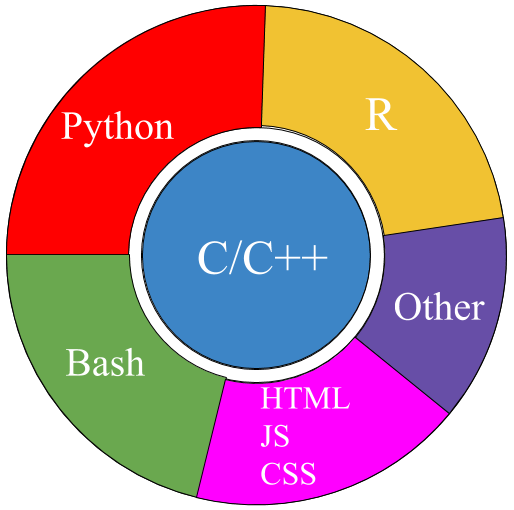
\includegraphics[scale=0.2]{img/programming.png}
    ~
  \section{OS Preference}
    \textbf{GNU/Linux}
\includegraphics[scale=0.40]{img/5stars.png}
    \textbf{Unix}
\includegraphics[scale=0.40]{img/4stars.png}
    \textbf{MacOS}
\includegraphics[scale=0.40]{img/3stars.png}
    \textbf{Windows}
\includegraphics[scale=0.40]{img/1stars.png}
    ~
\end{aside}



% \section{Person Statement}


\section{Experience}
\begin{entrylist}
  \entry
  {2018.12 - Now\\}
  {\large{Algorithm Engineer}}
  {Peng Chen Laboratory, Shenzhen, China}
  {Flight Control System Testing for fixed-wing UAV(Ardupilot), 3D Printing}

\end{entrylist}

\section{Education}
\begin{entrylist}

  \entry
    {2018.1 - 2018.11\\}
    {\large{Master of Research (Computer Science)}\\}
    {University of Wollongong, Australia}
    {Metamorphic Testing (Software Testing)\\
    \textbf{Main subjects}: Software Testing, Operational Research, Big Data
    Analysis, Natural Language Processing\\
    \textbf{Main Achievement}: \underline{One published paper}, Metamorphic Relations for Data Validation: A Case Study of Translated Text Messages}

  \entry
    {2014.3 - 2017.12\\}
    {\large{Bachelor of Computer Science}​}
    {University of Wollongong, Australia}
    {Major in Software Engineering\\
      \textbf{Main subjects}:\\
      Algorithms and Data Structures(80 Distinction)\\
      Object and Generic Programming in C++ (75 Distinction)\\
      Interactive Computer Graphics (75 Distinction)\\
      Multimedia Computing (73 Credit)\\
      software Engineering Practices \& Principles (82 Distinction)\\
      \textbf{Score Progress:}\\
      year 2014 avage score: 63.25\\
      year 2015 avage score: 45.14\\
      year 2016 avage score: 57.00 - final project got 82 distinction\\
      year 2017 avage score: 76.25 - distinction\\
      \textbf{Main Achievement}:\\
      1. The best final project prize ({\footnotesize Human Research Management System base on Web})\\
      2. First Three Semester had: Undergraduate Excellence Scholarship\\
    }
  \entry
  {2013.3 - 2014.3}
  {\large{English for Tertiary Studies}}
  {University of Wollongong College, Australia}
  {Main subjects: Academic English}

  \entry
    {2011.9 - 2013.3\\}
    {\large{Bachelor of Business Management}\\}
    {China University Of Mining And Technology}
    {Average mark of 91\% . Most of courses got High Distinction\\
    \textbf{Main subjects}: \\Mathematics 1: Algebra and Differential Calculus
    score: full mark\\Mathematics 2: Series and Integral Calculus score: 84}

\end{entrylist}

\newpage


\section{Publications}
Boyang Yan, Brian Yecies, Zhi Quan Zhou: Metamorphic Relations for Data
Validation: A Case Study of Translated Text Messages. IEEE/ACM 4th International
Workshop on Metamorphic Testing (MET '19), in conjunction with the 41st
International Conference on Software Engineering (ICSE '19), Montreal, Canada;
05/2019

\section{Academy Congress and Conference}
\begin{entrylist}
  \entry
  {May 26, 2019}
  {\\Paper Presentation - Title: Metamorphic Relations for Data Validation: A Case Study of Translated Text Messages}
  {ICSE, Montreal, Canada}

  \entry
  {August 11, 2017}
  {showing my final year project about Human Resource Management System based on
    Web (whole swap card subsystem and database are finish independently)\\}
  {IEEE Sections Congress (SC2017), Sydney, Australia}

\end{entrylist}

\section{Certifications}
\begin{entrylist}
  \entry
    {2017}
    {Amateur Radio Operator's certificate of proficiency (Standard)\\}
    {The Wireless Institute of Australia (WIA)}

  \entry
    {2016}
    {Ross a. Hull memorial Vhf-Uhf contest\\}
    {The Wireless Institute of Australia (WIA)}
    {Twelfth Place in Section A (Analog Modes, Best
7 Days) and Twelfth Place in Section C (Analog Modes, Best 2 Days)}

  \entry
    {2014}
    {Amateur Radio Operator's certificate of proficiency (Foundation)\\}
    {The Wireless Institute of Australia (WIA)}
   
  \entry
    {2010}
    {The Second Place Prize Awarded, Tianjin School Sports Competition Award "92" National Games Tianjin\\}
    {Tianjin Basketball Tryouts, China}
    {High school men's Group B. Primary and Secondary (Vocational) School Basketball Games. Have got the second grading certificate and title}

\end{entrylist}

\section{Training Courses}
\begin{entrylist}
  \entry
  {18.11.2018}
  {Sololearn(C++)}
  {Sololearn}

  \entry
  {2.9.2017}
  {Sololearn(Python3)}
  {Sololearn}

  \entry
    {2012}
    {Intel innovation in EDUCATION}
    {Intel Learn Program (Technical and Community)}

  \end{entrylist}

\begin{aside}
  \section{Languages}
    \textbf{Chinese}
\includegraphics[scale=0.40]{img/5stars.png}
    \textbf{English}
\includegraphics[scale=0.40]{img/4stars.png}
\end{aside}


\section{Extracurricular Activity}
I am a big fan of amateur radio (ham radio).
This is my biggest extracurricular activity.
In 2014, I have got my first amateur radio license (foundation license).
At that time, my purpose is talking and learning English because I can talk or send a message with all over the world radio amateur.
After my purpose is changed. I have found amateur radio have bigger relate with my major, computer science.
Amateur radio is not only sent morse code, which becomes history.
I am currently got my standard license.
So, I am more and more using new technology for radio.
Such as SSTV for the picture, D-STAR for digital mode voice transfer and data transfer.
Even International Space Station(ISS) also have got amateur radio FM repeater.
I am more and more focus on technique part for radio.
I also take part in some amateur radio competition.
For example, ross a. Hull memorial vhf-uhf contest.
I have got Twelfth Place in Section A (Analog Modes, Best 7 Days) and Twelfth Place in Section C (Analog Modes, Best 2 Days)).
This is only a part of my amateur radio activity.

\section{Research \& Project}
%\subsection*{\textcolor{blue}{Software Engineering Aspect}}
\begin{entrylist}
  \entry
  {2017}
  {Swap Card System\\}
  {University of Wollongong, Australia}
  {Swap card system for record attendance. I have using Arduino, raspberry pi,
    the level shifter, LCD controller and LCD screen. In raspberry pi, I have
    written by Python, using HTTP socket connect with Java backend. And using
    I2C bus connect with Raspberry Pi, Arduino and LCD controller. Level
    shifter for convert different volt in the I2C bus. RFID sense connects
    with Arduino. In Arduino, I have written by c++.}

  \entry
    {2017}
    {OPENGL construct a room\\}
    {University of Wollongong, Australia}
    {Using OPENGL construct a room with four walls and a floor, as well as two paintings, which are hung on separate walls, light, table and desk and so on.}

  \entry
    {2017}
    {OPENGL planetary system\\}
    {University of Wollongong, Australia}
    {OpenGL program for a planetary system
    \\\\ Github Link: \\{\small\url{https://github.com/yanboyang713/openGLPlanetarySystem.git}}}

  \entry
    {2016}
    {5th order low-pass Butterworth filter\\}
    {University of Wollongong, Australia}
    {Using SDL develop a program to process signal using the 5th order low-pass Butterworth filter and to play the processed signal.
     \\\\ Github Link: \\{\small\url{https://github.com/yanboyang713/butterworthFilter.git}}}

  \entry
    {2016}
    {image histogram equalization\\}
    {University of Wollongong, Australia}
    {Using SDL develop a colour image display and enhancement program. The program enhances an image using histogram equalization and displays the enhanced image.
     \\\\ Github Link:
     \\{\small\url{https://github.com/yanboyang713/histogramEqualizationImage.git}}}

    \entry
    {2018}
    {Metamorphic Testing in Text comparison tool\\}
    {University of Wollongong, Australia}
    {Using metamorphic testing method for testing DIFF utility quality. I have totally create 10 metamorphic relations.}

    \entry
    {2017}
    {Testing in machine translation software\\}
    {University of Wollongong, Australia}
    {Using metamorphic testing method for testing and compare Google, Bing and
      Youdao machine translation software quality.\\\\ Github Link:
      \\{\tiny\url{https://github.com/yanboyang713/Metamorphic-Testing-of-Machine-Translation-Software.git}}}

    \entry
    {2017}
    {Rainbow Table\\}
    {University of Wollongong, Australia}
    {Implementing a rainbow table for Anti-Hash Function write by c++
      \\\\ Github Link: \\{\small\url{https://github.com/yanboyang713/rainbowTable.git}}}

  \end{entrylist}

\section{Referral Info}
\begin{itemize}
	\item George Zhou <zhiquan@uow.edu.au> Research Project
	\item Jack Yang <jiey@uow.edu.au> Research Project
	\item Eve Shaw <eve@uow.edu.au> English aspect
	\item Mark Freeman <mfreeman@uow.edu.au> undergraduate final project
	\item Casey Chow <caseyc@uow.edu.au> computer graphics aspect
	\item Tianbing Xia <txia@uow.edu.au> base programming aspect and database aspect
\end{itemize}











\begin{flushleft}
  \today
\end{flushleft}
\begin{flushright}
\emph{Boyang Yan}
\end{flushright}

%%% This piece of code has been commented by Karol Kozioł due to biblatex errors. 
% 
%\printbibsection{article}{article in peer-reviewed journal}
%\begin{refsection}
%  \nocite{*}
%  \printbibliography[sorting=chronological, type=inproceedings, title={international peer-reviewed conferences/proceedings}, notkeyword={france}, heading=subbibliography]
%\end{refsection}
%\begin{refsection}
%  \nocite{*}
%  \printbibliography[sorting=chronological, type=inproceedings, title={local peer-reviewed conferences/proceedings}, keyword={france}, heading=subbibliography]
%\end{refsection}
%\printbibsection{misc}{other publications}
%\printbibsection{report}{research reports}

\end{document}
